\documentclass[tikz,border=1mm]{standalone}

\begin{document}
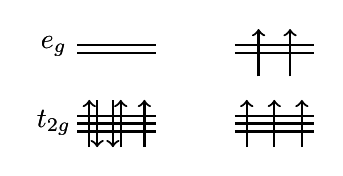
\begin{tikzpicture}
%low-spin eg
    \draw[thick] (-0.5,1) -- (0.5,1);
    \draw[thick] (-0.5,0.9) -- (0.5,0.9);

%low-spin t2g
    \draw[thick] (-0.5,0.1) -- (0.5,0.1);
    \draw[thick, ->] (-0.35,-0.3) -- (-0.35,0.3); %arrows
    \draw[thick, <-] (-0.25,-0.3) -- (-0.25,0.3); %arrows

    \draw[thick] (-0.5,0) -- (0.5,0);
    \draw[thick, ->] (0.05,-0.3) -- (0.05,0.3); %arrows
    \draw[thick, <-] (-0.05,-0.3) -- (-0.05,0.3); %arrows

    \draw[thick] (-0.5,-0.1) -- (0.5,-0.1);
    \draw[thick, ->] (0.35,-0.3) -- (0.35,0.3); %arrows

%low-spin labels
    \node[label={[xshift=-0.8cm, yshift=0.6cm] $e_{g}$}] {};
    \node[label={[xshift=-0.8cm, yshift=-0.4cm] $t_{2g}$}] {};

%high-spin eg
    \draw[thick] (1.5,1) -- (2.5,1);
    \draw[thick, ->] (1.8,0.6) -- (1.8,1.2); %arrows

    \draw[thick] (1.5,0.9) -- (2.5,0.9);
    \draw[thick, ->] (2.2,0.6) -- (2.2,1.2); %arrows

%high-spin t2g
    \draw[thick] (1.5,0.1) -- (2.5,0.1);
    \draw[thick, ->] (1.65,-0.3) -- (1.65,0.3); %arrows

    \draw[thick] (1.5,0) -- (2.5,0);
    \draw[thick, ->] (2,-0.3) -- (2,0.3); %arrows

    \draw[thick] (1.5,-0.1) -- (2.5,-0.1);
    \draw[thick, ->] (2.35,-0.3) -- (2.35,0.3); %arrows

%high-spin labels
    \node[label={[xshift=-0.8cm, yshift=0.6cm] $e_{g}$}] {};
    \node[label={[xshift=-0.8cm, yshift=-0.4cm] $t_{2g}$}] {};

\end{tikzpicture}
\end{document}

